\section{Cicli a gas e a vapore}
Una prima classificazione dei cicli termodinamici distingue tra cicli a gas e cicli a vapore.
L’analisi termodinamica dei cicli richiede la valutazione degli stati termodinamici dei punti
caratteristici del ciclo al fine di determinare le potenze termiche e meccaniche scambiate tra
macchina ciclica ed i serbatoi di calore e lavoro.
\subsection{Cicli a gas}
Le \textbf{formule semplificate} che mostriamo saranno \textbf{valide solo per cicli ideali}, nel momento in cui si analizzano \textbf{cicli reali} andranno usate le \textbf{definizioni}.\newline
\newline
Nei cicli termodinamici a gas faremo sempre l'ipotesi semplificativa di \textbf{gas perfetti}.\newline
\newline
Un ciclo termodinamico è rappresentato tipicamente da $4$ \textbf{politropiche}, uguali a due a due, per cui prendono il nome di \textbf{cicli simmetrici}.
\begin{center}
    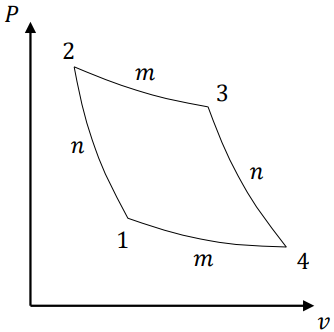
\includegraphics[height=4cm]{../L07/img1.PNG}
\end{center}
Nel caso di \textbf{ciclo ideale} (politropiche senza irreversibilità, cioè trasformazioni internamente seversibili) e ipotesi di \textbf{gas ideale}:
\[
    \begin{matrix}
        v_1v_3 = v_2v_4\\
        P_1P_3 = P_2P_4\\
        T_1T_3 = T_2T_4
    \end{matrix}
\]
(queste formule derivano dalla scrittura delle politropiche di ogni trasformazione e delle equazioni di stato dei gas ideali).\newline
\newline
Il termine $S_{irr}$ che abbiamo nel bilancio entropico può essere scomposto in $S_{irr,est}$, cioè le irreveribilità esterne (legate ai serbatoi e agli scambi), e $S_{irr, int}$, cioè le irreversibilità interne della macchina ciclica (irreversibilità delle trasformazioni). Nel caso ideale non avremo irreversibilità esterne, quindi nessuna irreversibilità nei serbatoi e negli scambi con la macchina ciclica. \newline
\newline
La maggior parte dei cicli hanno applicazioni per macchine motrici, alcuni però possono essere anche applicati a macchine operatrici.
\subsubsection{Ciclo di Carnot}
Il \textbf{ciclo di Carnot} è un \textbf{ciclo teorico} composto da 4 trasformazioni internamente reversibili, due \textbf{isoentropiche} e due \textbf{isoterme}.\newline
\newline
Questo ciclo rappresenta il ciclo ideale che si cerca di ottenere per una macchina per avere il rendimento massimo.\newline
\newline
\textbf{Rendimento}:
\[
    \eta = \frac{L}{Q_C} = 1- \frac{Q_F}{Q_C} = 1- \frac{T_{min}}{T_{max}}
\]
\ \newline
\textbf{Possibili fonti di irreversibilità}:
\begin{itemize}
    \item Irreversibilità esterne: $T_{min} > T_F$ e $T_{max} < T_C$;
    \item Irreversibilità interna: $s_1 > s_2$ e $s_3 < s_4$.
\end{itemize}
\subsubsection{Ciclo Joule-Brayton}
ciclo simmetrico a gas che nella sua realizzazione ideale è costituito da
due trasformazione \textbf{isoentropiche} e due trasformazioni \textbf{isobare}.\newline
\newline
Per il ciclo Joule Brayton viene definito il \textbf{rapporto delle pressioni}:
\[
    r_P = \frac{P_{max}}{P_{min}}
\]
mentre il \textbf{rendimento termodinamico} assume l'espressione:
\[
    \eta_{JB} = 1- \frac{T_1}{T_2} \;\;\;\;\;\;\;\;\;\;\eta_{JB} = 1- \frac{1}{r_P^{\frac{k-1}{k}}}
\]
con $k$ indice della politropica ($\frac{c_P}{c_V}$).\newline
Il rendimento è minimo quando la pressione $P_2$ tende alla presisone $P_1$ e quindi $r_{P,min} = 1$, mentre ha un valore massimo quanto $T_2$ tende a $T_3$ e quindi $r_{P,max} = \left(\frac{T_3}{T_1}\right)^{\frac{k}{k-1}}$.\newline
\newline
Il \textbf{lavoro specifico} nel caso di ciclo ideale e con gas perfetto vale:
\[
    l = c_P T_3 \left(1- \frac{T_4}{T_3}\right) - c_P T_1 \left(\frac{T_2}{T_1} - 1\right)
\]
\[
    l = c_P T_3 \left(1- \frac{1}{r_P^{\frac{k-1}{k}}}\right) - c_P T_1 \left(r_P^{\frac{k-1}{k}}-1\right)
\]
Per cui si ha il massimo lavoro specifico in corrispondenza del rapporto di compressione $r_{P,opt} = \left(\frac{T_3}{T_1}\right)^{\frac{k}{2(k-1)}} = \sqrt{r_{P,max}}$, che corrispone ha quanto $T_4 = T_2$, cioè nel momento in cui la temperatura di fine espansione coincide con quella di fine compressione.\newline
\newline
\newline
\newline
\textbf{Ciclo Joule-Brayton con rigenerazione}\newline
Rendimento del ciclo JB rigenerato \textbf{ideale} (in cui $T_{2'} = T_4$, cioè in cui si è recuperata tutta l'energia, e in cui si lavora con gas perfetti e il ciclo è ideale e simmetrico):
\[
    \eta_{rig} = \frac{\dot{L}}{\dot{Q}_C} = \frac{\dot{L}_T - \dot{L}_C}{\dot{Q}_C} = \frac{(T_3-T_4)-(T_2-T_1)}{(T_3-T_4)} = 1- \frac{T_2-T_1}{T_3-T_4}
\]
\[
    \eta_{rig} = 1- \frac{T_2}{T_3} = 1- \frac{T_2 T_1}{T_3T_1}
\]
\[
    \eta_{rig} = 1- \frac{T_1}{T_3}r_P^{\frac{k-1}{k}}
\]
In una rigenerazione \textbf{reale} si ha $T_{2'}< T_4$.
\subsubsection{Ciclo Otto}
ciclo simmetrico a gas che nella sua realizzazione ideale è costituito da due
trasformazione \textbf{isoentropiche} e due trasformazioni \textbf{isovolumiche} (isocore). \newline
\newline
Per il ciclo Otto (caso ideale simmetrico con gas perfetto) viene definito il \textbf{rapporto di compressione} volumetrico:
\[
    r_V = \frac{V_1}{V_2} = \frac{V_{max}}{V_{min}}
\]
mentre il \textbf{rendimento termodinamico} assume l'espressione:
\[
    \eta_{O} = 1- \frac{T_1}{T_2} \;\;\;\;\;\;\;\;\;\; \eta_{O} = 1- \frac{1}{r_V^{k-1}}
\]
\ \newline
Per il \textbf{lavoro specifico}:
\[
    l = c_V(T_3-T_4) -c_V(T_2-T_1)
\]
\[
    l = c_VT_3\left(1-\frac{T_4}{T_3}\right) - c_V T_1 \left(\frac{T_2}{T_1}-1 \right)
\]
\[
    l = c_V T_3 \left(1- \frac{1}{r_V^{k-1}}\right) - c_V T_1 (r_V^{k-1} - 1)
\]
Il lavoro è ottimale quando il rapporto di compressione vale
\[
    r_{V,opt} = \left(\frac{T_3}{T_1}\right)^{\frac{1}{2(k-1)}}
\]
\subsubsection{Ciclo Diesel}
ciclo non simmetrico a gas che nella sua realizzazione ideale è costituito da due
trasformazione \textbf{isoentropiche}, una trasformazione \textbf{isobara} e una trasformazioni \textbf{isovolumica}. \newline
\newline
Per il ciclo Diesel vengono definiti il \textbf{rapporto di compressione volumetrico} $r$ e il \textbf{rapporto di
combustione} $z$: 
\[
    r = \frac{V_1}{V_2} \;\;\;\text{che è uguale a dire }\; \frac{V_{max}}{V_{min}}
\]
\[
    z = \frac{V_3}{V_2} \;\;\;\text{che è uguale a dire}\; \frac{V_{fine \; combustione}}{V_{inizio \; combustione}}
\]
mentre il \textbf{rendimento termodinamico} assume l'espressione:
\[
    \eta = 1- \frac{1}{r^{k-1}} \frac{1}{k} \frac{(z^k - 1)}{(z-1)}
\]
\subsubsection{Ciclo Joule-Brayton inverso}
ciclo \textbf{frigorifero} (per macchine operatrici) simmetrico costituito da due \textbf{isoentropiche} e due \textbf{isobare}.\newline
\newline
L'\textbf{efficienza} del ciclo è data da
\[
    \epsilon = \frac{T_2}{T_3-T_2} = \frac{T_1}{T_4-T_1} = \left(\frac{1}{r_P^{\frac{k-1}{k}}}-1\right)
\]
\subsection{Cicli a vapore}
\subsubsection{Ciclo Rankine}
ciclo che nella sua realizzazione ideale è costituito da due trasformazione
\textbf{isoentropiche} e due trasformazioni \textbf{isobare}. Durante le due trasformazioni isobare si realizza
la transizione di fase. \newline
\newline
Il \textbf{rendimento termodinamico} è definito come:
\[
    \eta = \frac{\dot{L}}{\dot{Q}_C}
\]
\subsubsection{Ciclo frigorifero a vapore}
ciclo che nella sua realizzazione ideale è costituito da due
trasformazioni \textbf{isobare}, una trasformazione \textbf{isoentropica} e una trasformazione \textbf{isoentalpica
irreversibile}. \newline
\newline
L'\textbf{efficienza frigorifera} (detta anche $COP_F$) e l'\textbf{efficienza della pompa di calore} (detta anche $COP_{PC}$) sono definite come:
\[
    \epsilon_F = \frac{\dot{Q}_F}{\dot{L}} \;\;\;\;\;\;\;\;\;\;\epsilon_{PC} = \frac{\dot{Q}_C}{\dot{L}}
\]
Per l'analisi dei cicli termodinamici a vapore occorre utilizzare le tabelle termodinamiche con le proprietà delle sostanze.
\subsection{Osservazioni}
\begin{itemize}
    \item Per la determinazione del rendimento termodinamico di un ciclo non noto ci viene utile la definizione di rendimento nella forma:
    \[
        \eta = 1- \frac{Q_F}{Q_C}
    \]
    osservando che le trasformazioni per le quali, nel piano T- s, si ha un aumento di entropia
    comportano un trasferimento di calore alla macchina ciclica (calore entrante) mentre
    viceversa le trasformazioni per le quali si ha una riduzione di entropia sono associate a una
    cessione di calore dalla macchina ciclica. (es. isobara è calore entrante ($Q_C$), isocora è calore uscente ($Q_F$), le trasformazioni isoentropiche sono adiabatiche e quindi non hanno trasferimento di calore).
    \item  trasformazione \textbf{isoentropica} significa trasformazione adiabatica reversibile.
\end{itemize}